% Created by tikzDevice version 0.12.3.1 on 2023-01-22 16:55:02
% !TEX encoding = UTF-8 Unicode
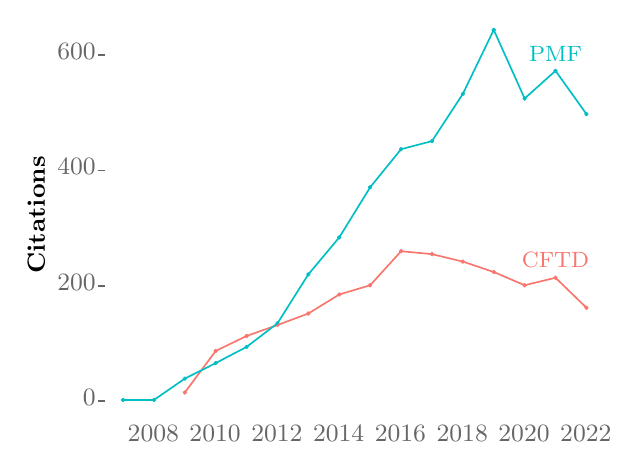
\begin{tikzpicture}[x=0.3pt,y=0.5pt]
%\path[draw,use as bounding box] (-50,0) rectangle (647,361.35);
\begin{scope}

\definecolor{drawColor}{RGB}{0,191,196}
\definecolor{fillColor}{RGB}{0,191,196}

\path[draw=drawColor,line width= 0.4pt,line join=round,line cap=round,fill=fillColor] ( 64.02, 57.87) ellipse [x radius=2,y radius=1.2];

\path[draw=drawColor,line width= 0.4pt,line join=round,line cap=round,fill=fillColor] (101.23, 57.87) ellipse [x radius=2,y radius=1.2];

\path[draw=drawColor,line width= 0.4pt,line join=round,line cap=round,fill=fillColor] (138.44, 73.28) ellipse [x radius=2,y radius=1.2];

\path[draw=drawColor,line width= 0.4pt,line join=round,line cap=round,fill=fillColor] (175.65, 84.53) ellipse [x radius=2,y radius=1.2];

\path[draw=drawColor,line width= 0.4pt,line join=round,line cap=round,fill=fillColor] (212.86, 96.19) ellipse [x radius=2,y radius=1.2];

\path[draw=drawColor,line width= 0.4pt,line join=round,line cap=round,fill=fillColor] (250.07,113.27) ellipse [x radius=2,y radius=1.2];

\path[draw=drawColor,line width= 0.4pt,line join=round,line cap=round,fill=fillColor] (287.28,148.68) ellipse [x radius=2,y radius=1.2];

\path[draw=drawColor,line width= 0.4pt,line join=round,line cap=round,fill=fillColor] (324.49,175.35) ellipse [x radius=2,y radius=1.2];

\path[draw=drawColor,line width= 0.4pt,line join=round,line cap=round,fill=fillColor] (361.70,211.59) ellipse [x radius=2,y radius=1.2];

\path[draw=drawColor,line width= 0.4pt,line join=round,line cap=round,fill=fillColor] (398.91,239.09) ellipse [x radius=2,y radius=1.2];

\path[draw=drawColor,line width= 0.4pt,line join=round,line cap=round,fill=fillColor] (436.12,244.92) ellipse [x radius=2,y radius=1.2];

\path[draw=drawColor,line width= 0.4pt,line join=round,line cap=round,fill=fillColor] (473.33,279.08) ellipse [x radius=2,y radius=1.2];

\path[draw=drawColor,line width= 0.4pt,line join=round,line cap=round,fill=fillColor] (510.54,325.32) ellipse [x radius=2,y radius=1.2];

\path[draw=drawColor,line width= 0.4pt,line join=round,line cap=round,fill=fillColor] (547.75,275.75) ellipse [x radius=2,y radius=1.2];

\path[draw=drawColor,line width= 0.4pt,line join=round,line cap=round,fill=fillColor] (584.96,295.74) ellipse [x radius=2,y radius=1.2] node[above,color=drawColor] {\footnotesize PMF};

\path[draw=drawColor,line width= 0.4pt,line join=round,line cap=round,fill=fillColor] (622.17,264.50) ellipse [x radius=2,y radius=1.2];
\definecolor{drawColor}{RGB}{248,118,109}
\definecolor{fillColor}{RGB}{248,118,109}

\path[draw=drawColor,line width= 0.4pt,line join=round,line cap=round,fill=fillColor] (138.44, 63.28) ellipse [x radius=2,y radius=1.2];

\path[draw=drawColor,line width= 0.4pt,line join=round,line cap=round,fill=fillColor] (175.65, 93.28) ellipse [x radius=2,y radius=1.2];

\path[draw=drawColor,line width= 0.4pt,line join=round,line cap=round,fill=fillColor] (212.86,104.11) ellipse [x radius=2,y radius=1.2];

\path[draw=drawColor,line width= 0.4pt,line join=round,line cap=round,fill=fillColor] (250.07,112.02) ellipse [x radius=2,y radius=1.2];

\path[draw=drawColor,line width= 0.4pt,line join=round,line cap=round,fill=fillColor] (287.28,120.36) ellipse [x radius=2,y radius=1.2];

\path[draw=drawColor,line width= 0.4pt,line join=round,line cap=round,fill=fillColor] (324.49,134.10) ellipse [x radius=2,y radius=1.2];

\path[draw=drawColor,line width= 0.4pt,line join=round,line cap=round,fill=fillColor] (361.70,140.77) ellipse [x radius=2,y radius=1.2];

\path[draw=drawColor,line width= 0.4pt,line join=round,line cap=round,fill=fillColor] (398.91,165.35) ellipse [x radius=2,y radius=1.2];

\path[draw=drawColor,line width= 0.4pt,line join=round,line cap=round,fill=fillColor] (436.12,163.26) ellipse [x radius=2,y radius=1.2];

\path[draw=drawColor,line width= 0.4pt,line join=round,line cap=round,fill=fillColor] (473.33,157.85) ellipse [x radius=2,y radius=1.2];

\path[draw=drawColor,line width= 0.4pt,line join=round,line cap=round,fill=fillColor] (510.54,150.35) ellipse [x radius=2,y radius=1.2];

\path[draw=drawColor,line width= 0.4pt,line join=round,line cap=round,fill=fillColor] (547.75,140.77) ellipse [x radius=2,y radius=1.2];

\path[draw=drawColor,line width= 0.4pt,line join=round,line cap=round,fill=fillColor] (584.96,146.18) ellipse [x radius=2,y radius=1.2] node[above,color=drawColor] {\footnotesize CFTD};

\path[draw=drawColor,line width= 0.4pt,line join=round,line cap=round,fill=fillColor] (622.17,124.52) ellipse [x radius=2,y radius=1.2];

\path[draw=drawColor,line width= 0.6pt,line join=round] (138.44, 63.28) --
	(175.65, 93.28) --
	(212.86,104.11) --
	(250.07,112.02) --
	(287.28,120.36) --
	(324.49,134.10) --
	(361.70,140.77) --
	(398.91,165.35) --
	(436.12,163.26) --
	(473.33,157.85) --
	(510.54,150.35) --
	(547.75,140.77) --
	(584.96,146.18) --
	(622.17,124.52);
\definecolor{drawColor}{RGB}{0,191,196}

\path[draw=drawColor,line width= 0.6pt,line join=round] ( 64.02, 57.87) --
	(101.23, 57.87) --
	(138.44, 73.28) --
	(175.65, 84.53) --
	(212.86, 96.19) --
	(250.07,113.27) --
	(287.28,148.68) --
	(324.49,175.35) --
	(361.70,211.59) --
	(398.91,239.09) --
	(436.12,244.92) --
	(473.33,279.08) --
	(510.54,325.32) --
	(547.75,275.75) --
	(584.96,295.74) --
	(622.17,264.50);
\end{scope}
\begin{scope}
\definecolor{drawColor}{gray}{0.4}

\node[text=drawColor,anchor=base east,inner sep=0pt, outer sep=0pt] at ( 31.16, 54.00) {\small 0};

\node[text=drawColor,anchor=base east,inner sep=0pt, outer sep=0pt] at ( 31.16,137.32) {\small 200};

\node[text=drawColor,anchor=base east,inner sep=0pt, outer sep=0pt] at ( 31.16,220.64) {\small 400};

\node[text=drawColor,anchor=base east,inner sep=0pt, outer sep=0pt] at ( 31.16,303.96) {\small 600};
\end{scope}
\begin{scope}
\definecolor{drawColor}{gray}{0.4}

\path[draw=drawColor,line width= 0.6pt,line join=round] ( 33.36, 57.03) --
	( 42.11, 57.03);

\path[draw=drawColor,line width= 0.6pt,line join=round] ( 33.36,140.35) --
	( 42.11,140.35);

\path[draw=drawColor,line width= 0.6pt,line join=round] ( 33.36,223.67) --
	( 42.11,223.67);

\path[draw=drawColor,line width= 0.6pt,line join=round] ( 33.36,306.99) --
	( 42.11,306.99);
\end{scope}

\begin{scope}
\definecolor{drawColor}{gray}{0.4}

%\node[text=drawColor,inner sep=0pt, outer sep=0pt] at ( 71.28, 33.41) {\small 2007}; rotate= 40.00,anchor=base east,

\node[text=drawColor,inner sep=0pt, outer sep=0pt] at (100.49, 33.41) {\small 2008};

%\node[text=drawColor,inner sep=0pt, outer sep=0pt] at (145.70, 33.41) {\small 2009};

\node[text=drawColor,inner sep=0pt, outer sep=0pt] at (174.91, 33.41) {\small 2010};

%\node[text=drawColor,inner sep=0pt, outer sep=0pt] at (220.12, 33.41) {\small 2011};

\node[text=drawColor,inner sep=0pt, outer sep=0pt] at (249.33, 33.41) {\small 2012};

%\node[text=drawColor,inner sep=0pt, outer sep=0pt] at (294.54, 33.41) {\small 2013};

\node[text=drawColor,inner sep=0pt, outer sep=0pt] at (323.75, 33.41) {\small 2014};

%\node[text=drawColor,inner sep=0pt, outer sep=0pt] at (368.96, 33.41) {\small 2015};

\node[text=drawColor,inner sep=0pt, outer sep=0pt] at (398.17, 33.41) {\small 2016};

%\node[text=drawColor,inner sep=0pt, outer sep=0pt] at (443.38, 33.41) {\small 2017};

\node[text=drawColor,inner sep=0pt, outer sep=0pt] at (472.59, 33.41) {\small 2018};

%\node[text=drawColor,inner sep=0pt, outer sep=0pt] at (517.80, 33.41) {\small 2019};

\node[text=drawColor,inner sep=0pt, outer sep=0pt] at (547.01, 33.41) {\small 2020};

%\node[text=drawColor,inner sep=0pt, outer sep=0pt] at (592.22, 33.41) {\small 2021};

\node[text=drawColor,inner sep=0pt, outer sep=0pt] at (621.43, 33.41) {\small 2022};
\end{scope}

\begin{scope}
\definecolor{drawColor}{RGB}{0,0,0}

\node[text=drawColor,rotate= 90.00,anchor=base,inner sep=0pt, outer sep=0pt] at ( -30,191.59) {\small \textbf{Citations}};
\end{scope}
\end{tikzpicture}